\documentclass[a4paper,10pt]{article}
\usepackage[utf8x]{inputenc}
\usepackage[hang]{subfigure}
\usepackage{graphicx}

\begin{document}

\begin{figure}[H]
\centering
\subfigure[The image to be filled. The target region is shown in green.]
  {
  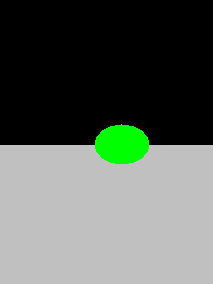
\includegraphics[width=0.3\linewidth]{BlackWhite}
  }
\subfigure[The naively computed gradient magnitude.]
  {
  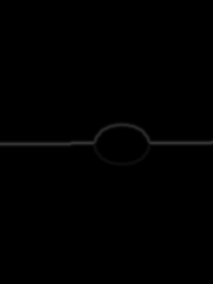
\includegraphics[width=0.3\linewidth]{ErroneousGradient}
  }
\subfigure[The gradient magnitude of the image with the slightly expanded hole.]
  {
  
\includegraphics[width=0.3\linewidth]{MaskedGradientMagnitude}
  }
\caption{The erroneous gradient problem.}
\end{figure}

\end{document}
